\documentclass{beamer}

\usefonttheme{professionalfonts} % using non standard fonts for beamer
\usefonttheme{serif} % default family is serif

\usepackage{hyperref}
%\usepackage{minted}
\usepackage{animate}
\usepackage{graphicx}
\def\Put(#1,#2)#3{\leavevmode\makebox(0,0){\put(#1,#2){#3}}}
\usepackage{colortbl}
\usepackage{tikz}
\usepackage{amssymb}
\usepackage{enumerate}
\usepackage{arydshln}
\usepackage{algorithm}
\usepackage{algpseudocode}

\colorlet{lightred}{red!25}
\colorlet{lightgreen}{green!25}
\beamertemplatenavigationsymbolsempty

\newcommand\blfootnote[1]{%
  \begingroup
  \renewcommand\thefootnote{}\footnote{#1}%
  \addtocounter{footnote}{-1}%
  \endgroup
}

\makeatletter

%% Textclass specific LaTeX commands.
\newcommand\makebeamertitle{\frame{\maketitle}}%
\AtBeginDocument{%
  \let\origtableofcontents=\tableofcontents
  \def\tableofcontents{\@ifnextchar[{\origtableofcontents}{\gobbletableofcontents}}
  \def\gobbletableofcontents#1{\origtableofcontents}
}
%% User specified LaTeX commands.
\usetheme{Malmoe}
\useoutertheme{infolines}
\addtobeamertemplate{headline}{}{\vskip2pt}
\setbeamercovered{transparent}

\makeatother

%%%%%%%%%%%%%%%%%%%%%%%%%%%%%%%%%%%%%%
%% Main document
%%%%%%%%%%%%%%%%%%%%%%%%%%%%%%%%%%%%%%
\begin{document}
\title[PFLOCK report]{PFLOCK Report}
\author[AC]{Andres Calderon}
\institute[Spring'20]{University of California, Riverside}
\makebeamertitle
\newif\iflattersubsect

\AtBeginSection[] {
    \begin{frame}<beamer>
    \frametitle{Outline} 
    \tableofcontents[currentsection]  
    \end{frame}
    \lattersubsectfalse
}

\AtBeginSubsection[] {
    \begin{frame}<beamer>
    \frametitle{Outline} 
    \tableofcontents[currentsubsection]  
    \end{frame}
}

\begin{frame}{Implementation done}
  \begin{itemize}
  \item The workflow was divided in two big jobs:
    \begin{enumerate}
    \item Finding pairs, centers and disks.
    \item Pruning redundant and duplicate disks (it required repartition).
    \end{enumerate}
  \item Run validations using LA\_50K and $\epsilon = 5m$.
    \item Average time = 2.96s
  \end{itemize}
  
\end{frame}

\begin{frame}{Candidate disks finding}{Task duration distribution}
  \centering
  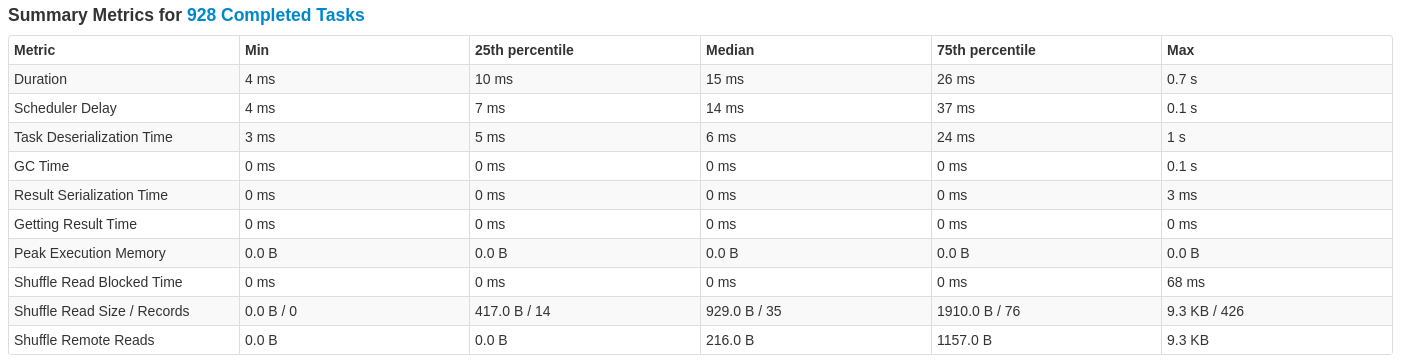
\includegraphics[width=\textwidth]{figures/Stage4Summary}
\end{frame}

\begin{frame}{Candidate disks finding}{Node load distribution}
  \centering
  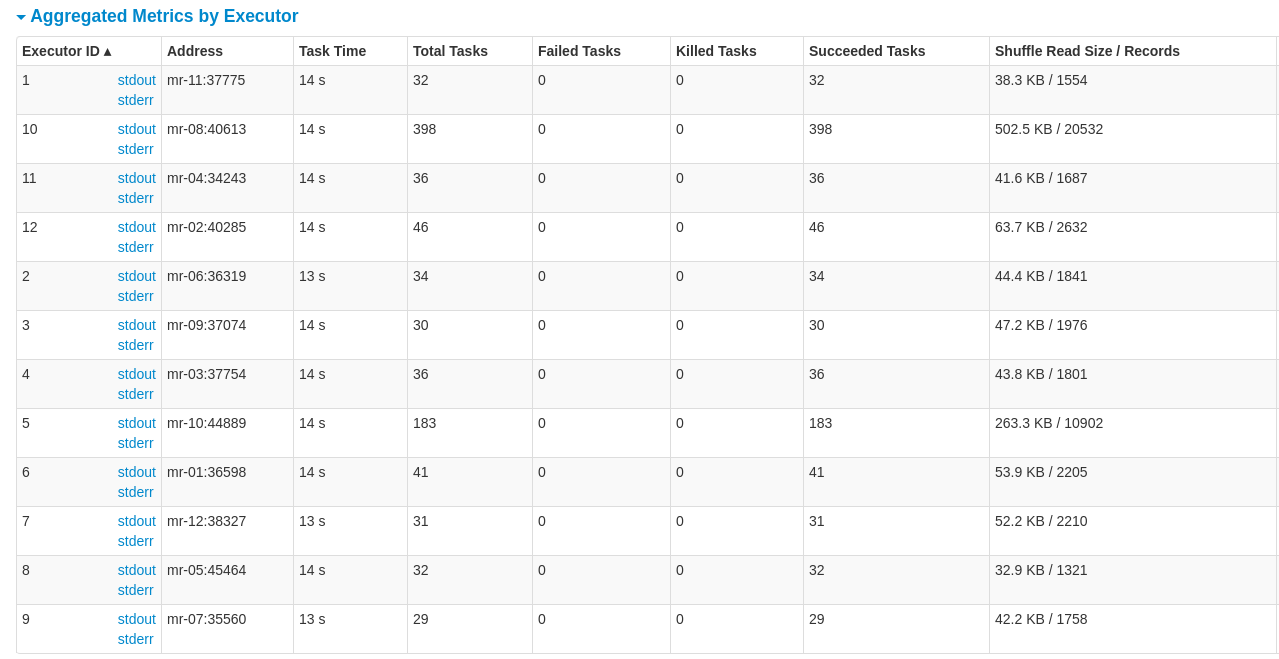
\includegraphics[width=\textwidth]{figures/Stage4ByExecutor}
\end{frame}

\begin{frame}{LCM pruning}{Task duration distribution}
  \centering
  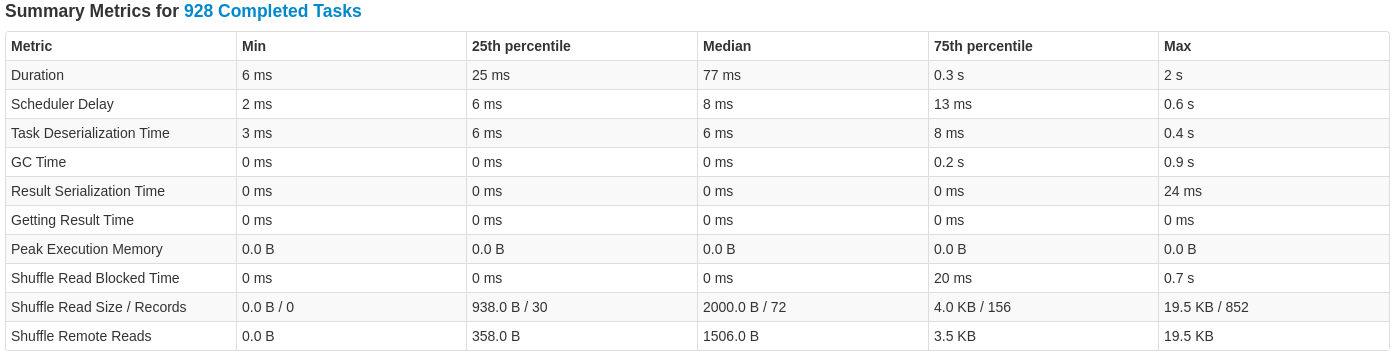
\includegraphics[width=\textwidth]{figures/Stage7Summary}
\end{frame}

\begin{frame}{LCM pruning}{Node load distribution}
  \centering
  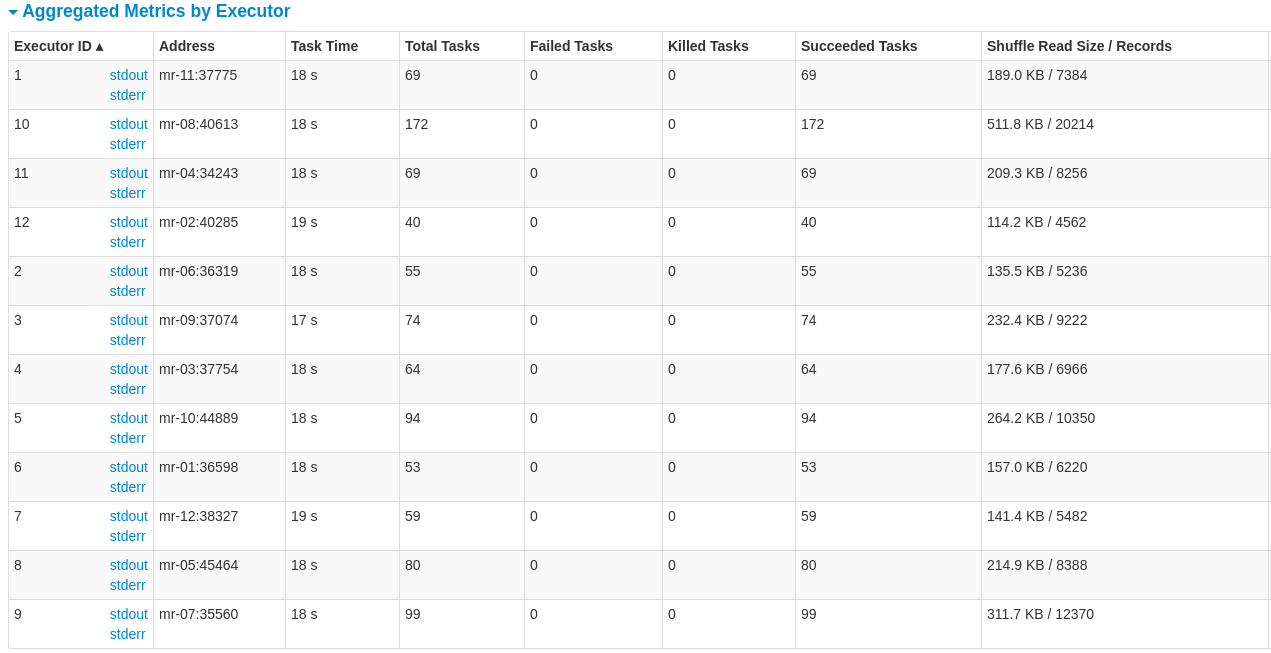
\includegraphics[width=\textwidth]{figures/Stage7ByExecutor}
\end{frame}

\begin{frame}{What's next}
    \begin{itemize}
      \item Dealing with some minor bugs.
      \item Completing experiments and plot the results.
    \end{itemize}
\end{frame}

\end{document}

